\documentclass{beamer}
\usepackage{graphicx} % Required for inserting images

\usepackage[utf8]{inputenc}
\usepackage[T1]{fontenc}
\usepackage{lmodern}
\usepackage{amsmath,amssymb}
\usepackage{microtype}
\usepackage{ellipsis}
%\usepackage[ngerman]{babel}
\let\openbox\undefined
\usepackage{mathtools}
\usepackage{enumitem}
\let\openbox\undefined
\usepackage{amsthm}
\usepackage{thmtools}
\usepackage{graphicx}
\usepackage{stmaryrd}
\usepackage{tikz}
\usetikzlibrary{positioning}
\usepackage{algpseudocode}
\usepackage[absolute,overlay]{textpos}
\usepackage{url}
\usepackage[
backend=biber,
style=numeric,
]{biblatex}
\addbibresource{references.bib}
\usepackage[normalem]{ulem}
\usepackage{verbatim}
\usepackage{subcaption} % allow for subfigures

\usepackage[ruled, algosection]{algorithm2e}


\declaretheoremstyle[
  spaceabove=\parsep,
  spacebelow=0,
  headfont=\bfseries,
  notefont=\bfseries,
  notebraces={(}{)},
  bodyfont=\normalfont,
  postheadspace=.5em
]{definition}

\newtheoremstyle{plain}         % name
    {\parsep}                   % Space above
    {}                          % Space below
    {}                          % Body font
    {}                          % Indent amount
    {\bfseries}                 % Theorem head font
    {.}                         % Punctuation after theorem head
    {.5em}                      % Space after theorem head
    {\thmname{#1}\thmnumber{ #2}\thmnote{ \bfseries (#3)}}                 % Theorem head spec (can be left empty, meaning ‘normal’)

\theoremstyle{plain}

% \declaretheorem[sharenumber=algocf]{theorem}
% \declaretheorem[sharenumber=algocf]{lemma}
% \declaretheorem[sharenumber=algocf]{corollary}
\declaretheorem[sharenumber=algocf]{proposition}

% \declaretheorem[sharenumber=algocf]{definition}
% \declaretheorem[sharenumber=algocf]{example}
\declaretheorem[sharenumber=algocf]{remark}
\declaretheorem[sharenumber=algocf]{notation}

\renewcommand\qedsymbol{$\square$}

\newcommand\R{\mathbb R}
\newcommand\Z{\mathbb Z}
\newcommand\N{\mathbb N}
\newcommand\C{\mathbb C}
\newcommand{\Q}{\mathbb Q}
\newcommand{\F}{\mathbb{F}}
\newcommand{\ass}{\underline{Assume:}  }
\newcommand{\zz}{\underline{t.s.:}  }

\renewcommand{\phi}{\varphi}
\renewcommand{\epsilon}{\varepsilon}


\newcommand{\stab}{\mathrm{Stab}}
\newcommand{\conv}{\mathrm{conv}}
\newcommand{\vol}{\mathrm{vol}}
% \newcommand{\min}{\text{min}}
% \newcommand{\max}{\text{max}}
% \newcommand{\ker}{\text{ker}}
\newcommand{\im}{{\mathrm{im}}}
\newcommand{\GL}{\mathrm{GL}}
\newcommand{\Aut}{{\mathrm{Aut}}}

\newcommand{\T}{\mathcal{T}}
\renewcommand{\P}{\mathcal{P}}
\renewcommand{\L}{\mathcal{L}}

\usetheme[compress]{Berlin}
\setbeamertemplate{footline}[frame number]{}
\setbeamertemplate{navigation symbols}{}
\setbeamertemplate{footline}{}

\makeatletter
\beamer@theme@subsectionfalse%
\makeatother


\title{Berechnung von Dirichletzellen kristallographischer Gruppen mittels endlicher Wortlänge }
% \subtitle{With connections to topological interlocking}
\author{Lukas Schnelle}
\date{Grüppchen 2025 \\ In Zusammenarbeit mit \\Alice C. Niemeyer und Reymond Akpanya}


\begin{document}

% remove dots on first slide
\frame[plain]{\titlepage}

\section{Kristallographische Gruppen}
\begin{frame}
    In diesem Vortrag operieren wir von rechts, also z.B. ein Gruppenelement $\phi \in G$ einer Gruppe $G$ die auf einer Menge $M$ operiert, wird bezeichnet als $m^\phi$ für $m \in M$.
    \pause
    \begin{notation}
        Seien $v, w \in \R^n$ Vektoren und $r \in \R$ eine reelle Zahl. \pause 
        Dann bezeichnen wir mit 
        \begin{enumerate}[label=(\roman*)]
            \item $\langle v, w \rangle$ das Euklidische Skalarprodukt,\pause
            \item $||v|| \coloneqq \sqrt{\langle v, v \rangle}$ die Euklidische Norm,\pause
            \item $d(v, w) \coloneqq ||v - w ||$ die Euklidische Distanz,\pause
            \item $B_r(v) \coloneqq \{ u \in \R^n \mid d(v, u) < r \}$ den offenen $r$-Ball und mit \pause
            \item $\overline{B_r(v)} \coloneqq \{ u \in \R^n \mid d(v, u) \leq r \}$ den abgeschlossenen $r$-Ball. 
        \end{enumerate}  
    \end{notation}
    \pause
    Kurz: Unsere Welt ist eine Euklidische.
\end{frame}

\begin{frame}
    \begin{definition}
        Sei $n \in \N$ und $\phi: \R^n \to \R^n$. Dann bezeichnen wir $\phi$ also \emph{Isometrie}, falls für alle $v, w \in R^n$ gilt, dass:
        $$
            d(v^\phi, w^\phi) = d(v, w).
        $$\pause
        Die Menge aller Isometrien zu einem festen $n$ bezeichnen wir mit $E(n)$.
    \end{definition}
    \pause
    \begin{proposition}
        Sei $n \in \N$ fest. Dann ist die Menge aller Isometrien $E(n)$ eine Gruppe mit der Konkatenation von Abbildungen als Gruppenoperation.
        Diese Gruppe bezeichnen wir als die \emph{euklidische Gruppe}. Die Gruppe operiert auf $\R^n$ durch die Anwendung eines Gruppenelements als Abbildung.
    \end{proposition}
\end{frame}
% Bsp?
% system of representatives
\begin{frame}
    \begin{definition}
        Sei $\Gamma \leq E(n)$ eine Untergruppe und $F \subseteq \R^n$ eine abgeschlossene Menge. Dann heißt $F$ ein \emph{Fundamentalbereich} von $\Gamma$ falls
        \begin{enumerate}[label=(\roman*)]
            \item $\bigcup_{\gamma \in \Gamma} F^\gamma = \R^n$\pause
            \item es gibt ein Vertretersystem $V \subseteq \R^n$ von den Bahnen der Operation von $\Gamma$ auf $\R^n$, sodass
                $$
                    F^\circ \subseteq V \subseteq F.
                $$
        \end{enumerate}
    \end{definition}

    \pause
    \begin{definition}
        Sei $\Gamma \leq E(n)$ eine Untergruppe. Dann heißt $\Gamma$ kristallographische Gruppe falls $\Gamma$ eine diskrete Untergruppe ist und ein kompakter Fundamentalbereich von $\Gamma$ existiert.
    \end{definition}
    In der Literatur werden kristallographische Gruppen (insbesondere der Dimension $3$) auch als Raumgruppen bezeichnet.
\end{frame}

\begin{frame}
    In 1900 hat Hilbert 23 Probleme bei einem Kongress vorgestellt, die zu diesem Zeitpunkt ungelöst waren.
    \begin{block}{18. Hilbert Problem}
        Gibt es für festes $n$ endlich viele kristallographische Gruppen?
    \end{block}
    \pause
    \begin{exampleblock}{Bieberbachsche Sätze (1910)}
        Ja, für festes $n \in \N$ gibt es nur endlich viele kristallographische Gruppen. \\
        Für $n=2$ gibt es $17$, für $n=3$ gibt es $230$.
    \end{exampleblock}
    Für bis niedrige Dimensionen sind alle dieser Gruppen bekannt, z.B. für $n\leq 4$ hier: \cite{crystGrpsDimFour}.
\end{frame}

\begin{frame}
    \centering
    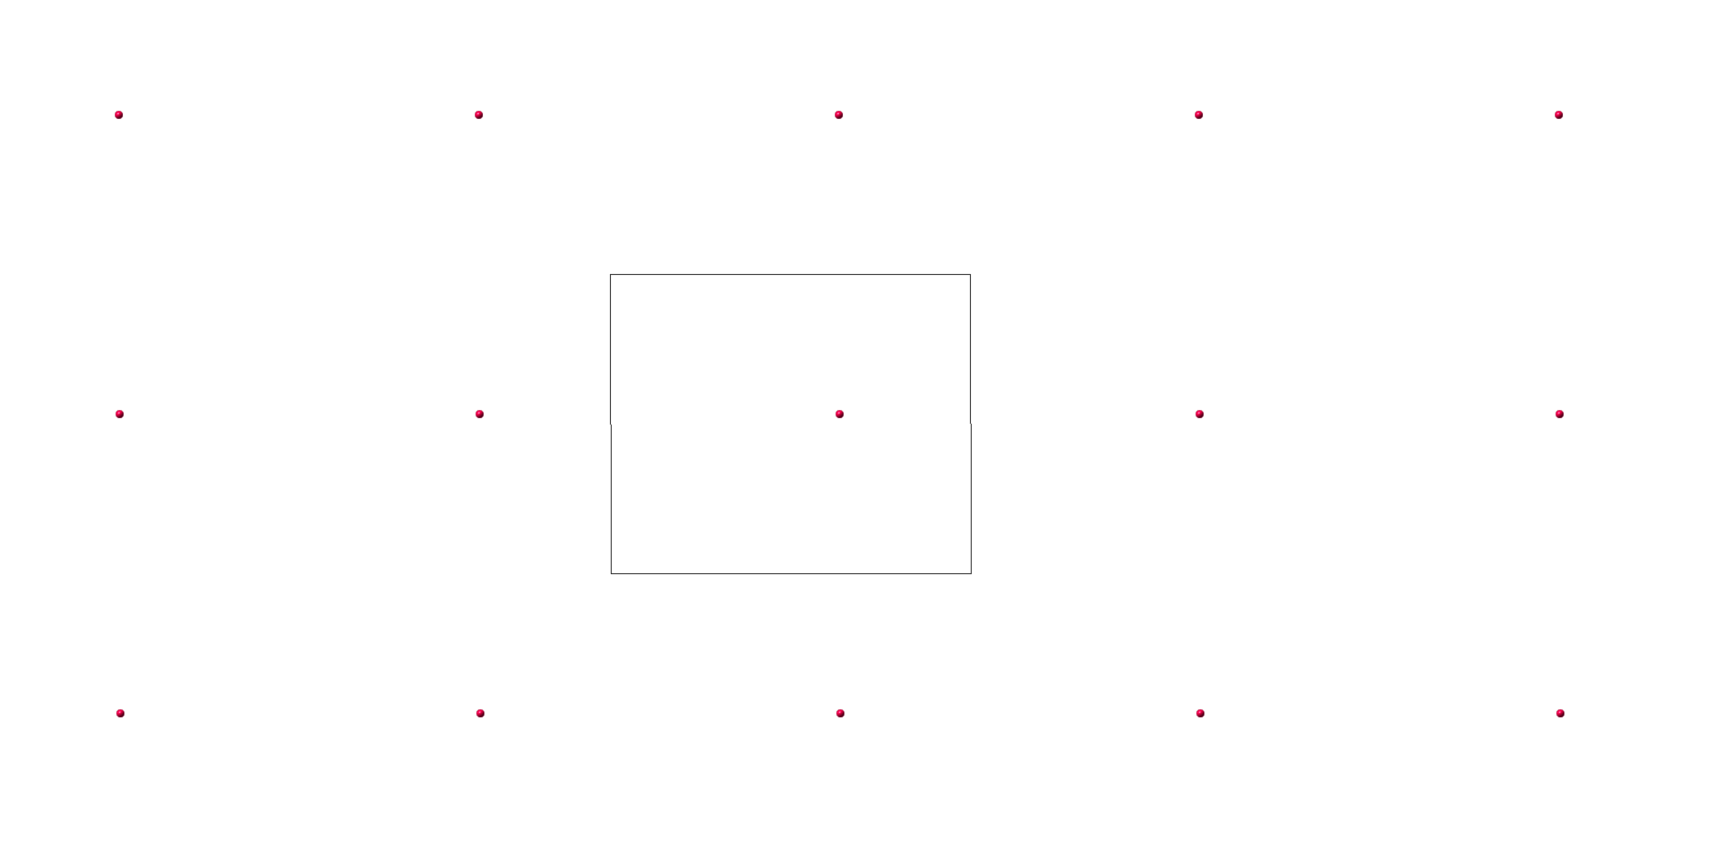
\includegraphics[width=\textwidth]{images/p1-escher.png}
\end{frame}

\begin{frame}
    \centering
    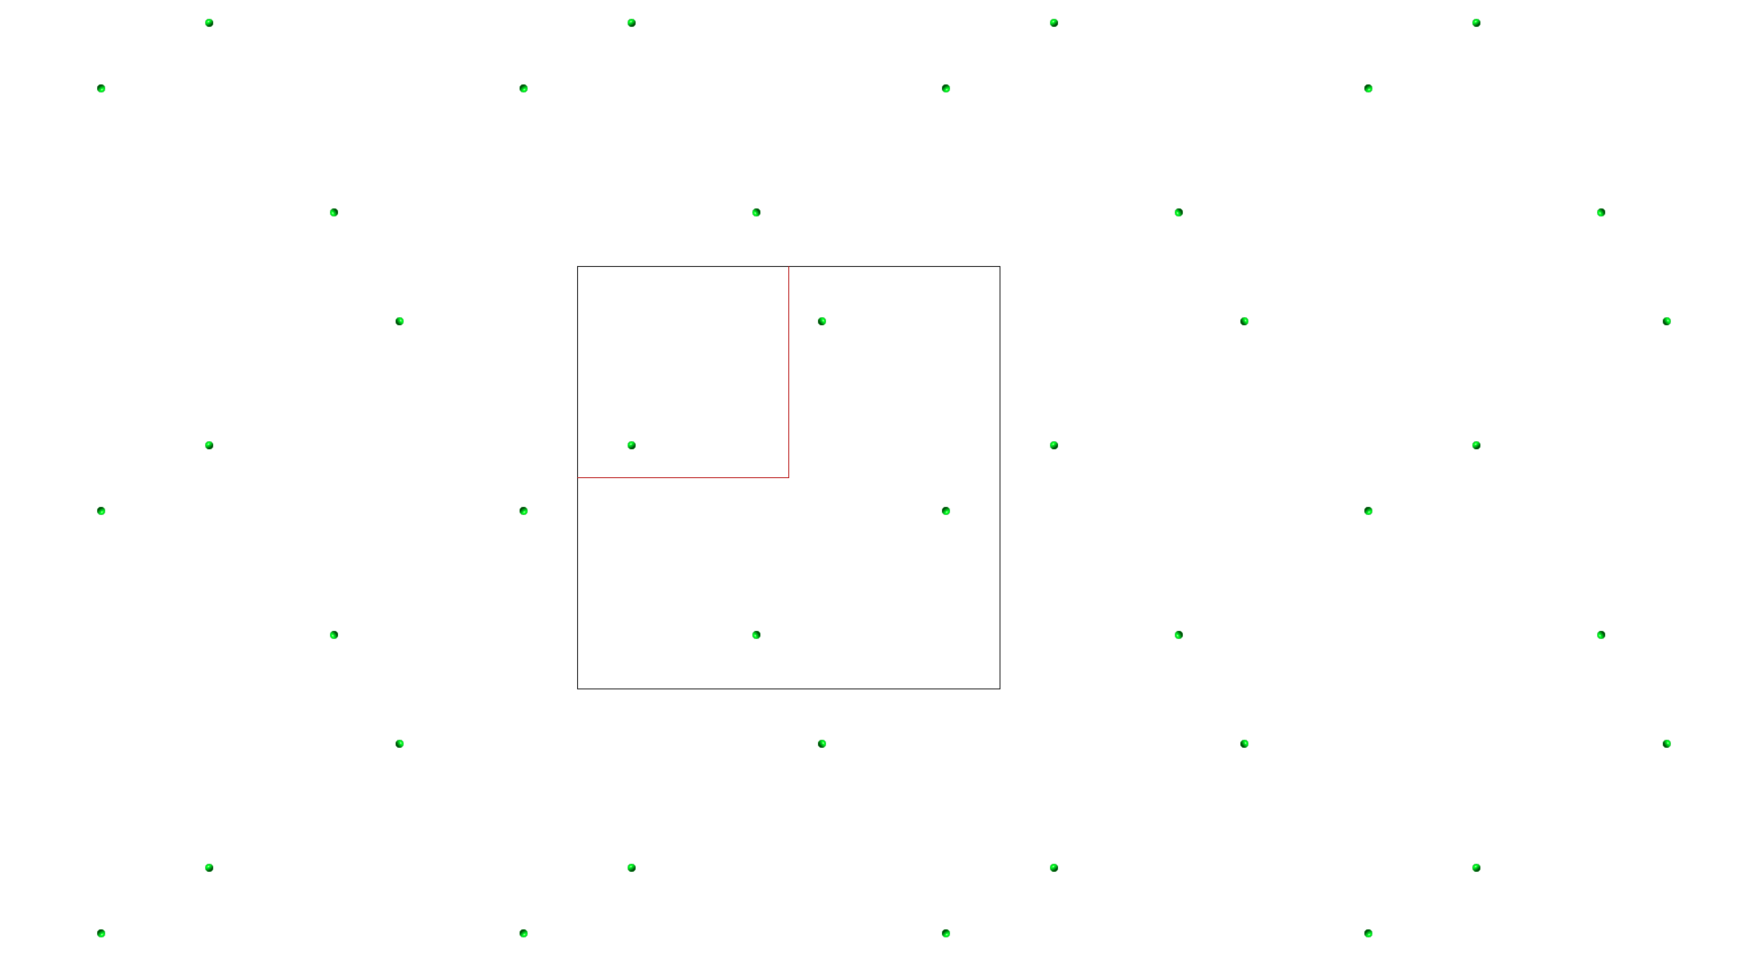
\includegraphics[width=\textwidth]{images/p4-escher.png}
\end{frame}


\section{Dirichletzellen}
\begin{frame}
    \begin{alertblock}{Problem}
        Gegeben eine kristallographische Gruppe $\Gamma \leq E(n)$. Was ist ein Fundamentalbereich?
    \end{alertblock}
    \pause
    \begin{exampleblock}{Antwort}
        Dirichletzellen
    \end{exampleblock}
\end{frame}

\begin{frame}
    \begin{definition}
        Seien $u, v \in \R^n$ Vektoren. Wir nennen
        $$
            H^+(u, v) \coloneqq \{ w \in \R^n \mid d(u,w) \leq d(v, w) \}
        $$
        den \emph{Halbraum} von $u$ und $v$.
    \end{definition}
    \pause
    \begin{definition}
        Sei $O \subseteq \R^n$ eine diskrete Menge und $u \in O$ ein Punkt.
        Dann nennen wir 
        $$
		    D(u, O) \coloneqq \{ v \in \R^n \mid \forall w \in O \setminus \{ u \} : d(u, v) \leq d(v, w) \}
	    $$
        die \emph{Dirichletzelle} von $u$ und $O$.
    \end{definition} \pause
    Oft nutzen wir die äquivalente Formulierung
    $$
		D(u, O) = \bigcap_{w \in O, w \neq u} H^+(u, w).
	$$
\end{frame}

\begin{frame}
    \centering
    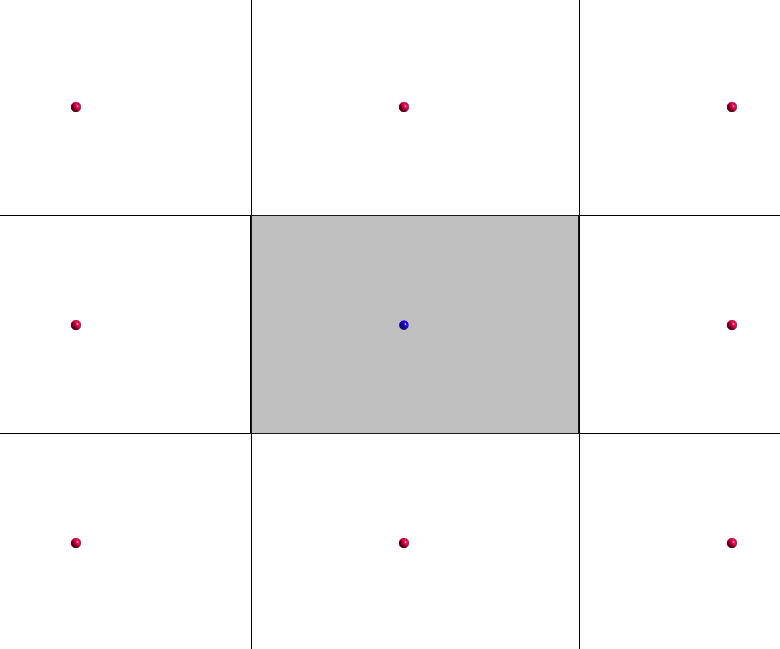
\includegraphics[width=0.7\textwidth]{images/dirichlet-example.png}
\end{frame}

\begin{frame}
    \begin{definition}
        Sei $\Gamma \leq E(n)$ eine kristallographische Gruppe und $v \in \R^n$ ein Vektor.
        Wir nennen $v$ in \emph{spezieller Lage} bzgl. $\Gamma$, falls 
        $$
            Stab_\Gamma(v) \neq \{Id\},
        $$
        sonst nennen wir ihn in \emph{allgemeiner Lage}.
    \end{definition}
    \pause
    \begin{theorem}[{\cite[Thm. III.11 (ii)]{plesken1994}}]
        Sei $\Gamma \leq E(n)$ eine kristallographische Gruppe und $u \in \R^n$ in allgemeiner Lage. Dann ist $D(u, u^\Gamma)$ ein Fundamentalbereich von $\Gamma$.
    \end{theorem}
    \pause
    Erinnerung:
    $$
		D(u, O) = \bigcap_{w \in O, w \neq u} H^+(u, w).
	$$
\end{frame}

\begin{frame}
    \centering
    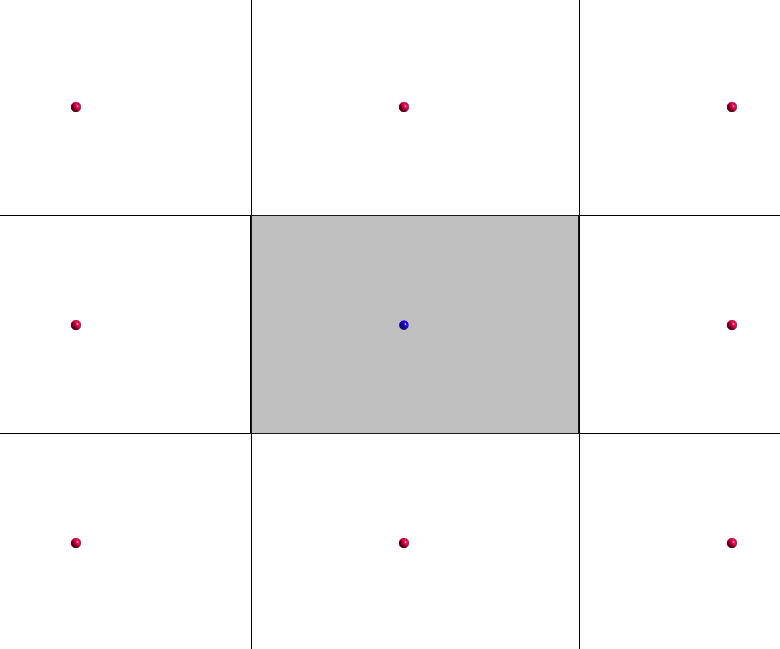
\includegraphics[width=0.7\textwidth]{images/dirichlet-example.png}
\end{frame}

\begin{frame}
    \begin{alertblock}{Problem}
        $u^\Gamma$ ist unendlich.
    \end{alertblock}
\end{frame}

\begin{frame}
    \begin{block}{Idee}
        Halbräume die von zwei weit entfernten Punkten aufgespannt werden, haben weniger Einfluss als Halbräume, die von nahe beieinander liegenden Punkten aufgespannt werden.
    \end{block}
    \pause
    \begin{block}{Ansatz}
        Betrachte nur Isometrien, die einen Punkt nicht "zu weit weg" operieren.
    \end{block}
\end{frame}

\begin{frame}
    fsdfsd
\end{frame}

\section{Endliche Wortlänge}

\section{Motivation}

\begin{frame}
    \printbibliography
\end{frame}

\end{document}
